\renewcommand{\chaptername}{Feb 8th: Lab}
\chapter{Quantum Confinement and Superposition}
In quantum mechanics, particles can be 'spatially confined' to a given energy potential where the energy levels of the confined particles will not remain continuous (as in the case of bulk materials) but instead are now quantized.
Quantum mechanics allows us to obtain the wave functions of the confined particle and their discrete set of energy levels -- such kinds of effects appear when the dimensions of the potential approach the deBroglie wavelength of particle. These effects are the basis for several semiconductor devices, including nano-crystals often called quantum dots.
In this lab, the following objectives were pursued:
\begin{itemize}
    \item Visualise the energy levels of a confined particle as well as the behaviour of its quantum wavefunction,
    \item Obtain deeper understanding and visualise the nature of qunatum superposition.
\end{itemize}

The infinite square well (often called ``particle in a box'') provides several illustrations of the properties of wave functions whilst being one of the less troublesome problems to solve. This can be done using the time-independent, one-dimensional Schrödinger equation.

\begin{figure}[h]
    \centering
    
\includegraphics[width=0.3\textwidth]{frog.jpg} %particleInABox
    \caption{Particle in a Box}
    \label{fig:particleInABox}
\end{figure}

This problem requires that we set a potential, which we can make:

\[
  V(x) = \begin{cases}
  0 & 0 < L < 1\\
  \infty & \text{elsewhere}
\end{cases}
\]


Although this potential is clearly artificial, the problem is worth carefully studying for several reasons: 
\begin{itemize}
    \item Exact solutions to the Schrödinger equation can be obtained without the difficult mathematics which usually accompanies its solution for more realistic potential functions,
    \item The problem is closely related to many familiar classical problems,
    \item It illustrates many of the important features of all quantum-mechanics problems,
    \item This potential is a relatively good approximation to some real situations.
\end{itemize}

\section{Methods}
   
These properties were inspected in detail using \textbf{Python}.
   
\section{Results}

Derivation of energy equation to calculate the quantised energies:

Consider the time-independent, one-dimensional Schrödinger equation in the $x$ direction:

$$E_n \Psi_n (x) = \frac{-\hbar ^{2}}{2m}\frac{\delta^{2}}{\delta x^{2}}\Psi_n (x) + V(x)\Psi_n (x)$$

where $\hbar$ is some fucking Planck Constant, $m$ is the mass of the particle, $a$ is the length of the \textbf{well?}, $\Psi_n (x)$ is the wavefunction, $V(x)$ is the potential and $E_n$ is the energy level. 

$V(x)$ in the potential well = 0: 

\begin{equation} \label{eq:1}
E_n \Psi_n (x) = \frac{-\hbar ^{2}}{2m}\frac{\delta^{2}}{\delta x^{2}}\Psi_n (x)
\end{equation}


Substituting $\Psi_n (x)$ for its \textbf{eigenfunction}:

$$E_n \Psi_n (x) = \frac{-\hbar ^{2}}{2m}\frac{\delta^{2}}{\delta x^{2}}\Bigg(\sqrt{\frac{2}{a}}\sin\Big(\frac{n\pi x}{a}\Big)\Bigg)$$

$$E_n \Psi_n (x) = \frac{-\hbar ^{2}}{2m}\Big(\frac{n\pi}{a}\Big)^{2}\Bigg(\sqrt{\frac{2}{a}}\sin\Big(\frac{n\pi x}{a}\Big)\Bigg)$$

$$E_n \Psi_n (x) = \frac{\hbar ^{2}}{2m}\Big(\frac{n\pi}{a}\Big)^{2}\Psi_n (x)$$

$$E_n = \frac{\hbar ^{2}}{2m}\Big(\frac{n\pi}{a}\Big)^{2} \quad \quad \quad \text{where } n \in \mathbb{N}$$

The quantised energy values (energy eigenvalues) for a box 0.1nm in width (a=0.1nm) for $n=1$ to $n=5$ are plotted below:

\begin{figure}[h]
    \centering
    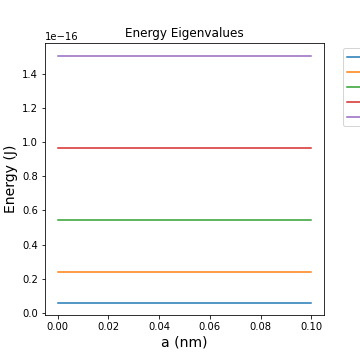
\includegraphics[width=0.75\textwidth]{lab1/eigenvaluesEnergy.png}
    \caption{Plot showing the discrete energy levels for a particle in a box of length 0.1nm. First 5 energy levels are show (n=1 to n=5)}
    \label{fig:eigenEnergy}
\end{figure}

Table \ref{tab:qEnerergy} shows the values for these quantised energies:

Substituting $n=1$:
$$E_1 = \frac{\hbar ^{2}\pi^{2}}{2ma^{2}}$$

\begin{equation}\label{eq:energySpacing}
\implies E_n =  n^{2}E_1
\end{equation}




\begin{table}[h!]
\centering
\begin{tabular}{|l|l|l|}
\hline
\textbf{n} & \textbf{Energy (J)} \\ \hline
1 & 6.02467e-18 \\ \hline
2 & 2.40987e-17 \\ \hline
3 & 5.42220e-17 \\ \hline
4 & 9.63946e-17 \\ \hline
5 & 1.50617e-16 \\ \hline
\end{tabular}
%\captionsetup{font = it, labelfont = bf, width=.91\linewidth, justification=centering}
\caption{\textit{Table showing the calculated energy states of an electron confined in a one dimensional box with $L=0.1nm$}}
\label{tab:qEnerergy}
\end{table}

Calculating the normalised wavefunction = eigenfunction:

Rearranging Equation \ref{eq:1}:

$$\frac{\delta^{2}}{\delta x^{2}}\Psi_n (x) = \frac{-2m}{\hbar} E \Psi_n (x) = -k^2 \Psi_n (x)$$

where $k=\frac{-2m}{\hbar}$.

The general equation must follow the following expression:

$$\Psi_n (x) = A \sin(kx) + B cos(kx)$$ %DO YOU INCLUDE THE SUBSCRIPT N?

Applying the boundary condition, $\Psi_n (x)$=0 at x=0:
$$\implies 0 = A sin(0) + B cos(0)$$
$$ 0 = B$$
$$\therefore \Psi_n (x) = A sin(x)$$

Applying the boundary condition, $\Psi_n (x)$=0 at x=a:
$$\implies 0 = A sin(ka)$$ %WHERE DID K COME FROM?!
$$ ka = \pi n \quad \text{where } n \in \mathbb{N}$$
$$ k = \frac{\pi n}{a}$$
$$\therefore \Psi_n (x) = A sin(\frac{\pi n}{a}x)$$

A must satisfy the following normalised:

$$\int_{ -\infty}^{\infty}\Psi_n (x)^{*}\Psi_n (x)dx = 1$$
$$\int_{ -\infty}^{0}\Psi_n (x)^{*}\Psi_n (x)dx +\int_{0}^{a}\Psi_n (x)^{*}\Psi_n (x)dx + \int_{ a}^{\infty}\Psi_n (x)^{*}\Psi_n (x)dx= 1$$
$$\int_{ 0}^{a} A^{*} [sin(\frac{\pi n}{a}x)]^{*}A sin(\frac{\pi n}{a}x)dx = 1$$
$$A^{*}A\int_{ 0}^{a} [sin(\frac{\pi n}{a}x)]^{*}sin(\frac{\pi n}{a}x)dx = 1$$
$$\left | A \right |^2 \int_{ 0}^{a} sin(\frac{\pi n}{a}x) sin(\frac{\pi n}{a}x)dx = 1$$
$$\left | A \right |^2 \int_{ 0}^{a} sin^{2}(\frac{\pi n}{a}x)dx = 1$$
$$\left | A \right |^2 \left[\frac{x}{2}-\frac{asin(\frac{2 \pi nx}{a})}{4 \pi n}\right]_0^a= 1$$
$$\left | A \right |^2 [(\frac{a}{2}-0)-(0-0)]= 1$$
$$\left | A \right |^2 \frac{a}{2}= 1$$
$$\left | A \right | = \sqrt{\frac{2}{a}}$$
$$\therefore \Psi_n (x) = \sqrt{\frac{2}{a}} sin(\frac{\pi n}{a}x)$$ %MAGNITUDE?!

Figure \ref{fig:normWave} shows plots of the wavefunctions $\psi_n(x)$ and Figure \ref{fig:probDens} probability densities $P_n(x)$ for $n=1$ to $n=5$. 
 
\begin{figure}[h]
    \centering
    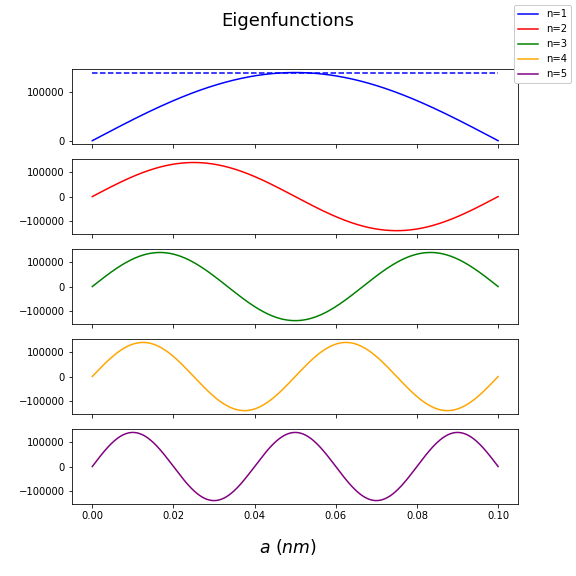
\includegraphics[width=0.6\textwidth]{lab1/normalisedWavefunction.png}
    \caption{Normalised wavefunction for n=1 to n=5}
    \label{fig:normWave}
\end{figure}

Then plotted the probability density functions (PDFs), $P_n (x)$, given by:

$$P_n(x) = |\Psi_n(x)|^{2} = \Bigg|\sqrt{\frac{2}{a}}\sin\Big(\frac{n\pi x}{a}\Big)\Bigg|^{2}  $$

\begin{figure}[h]
    \centering
    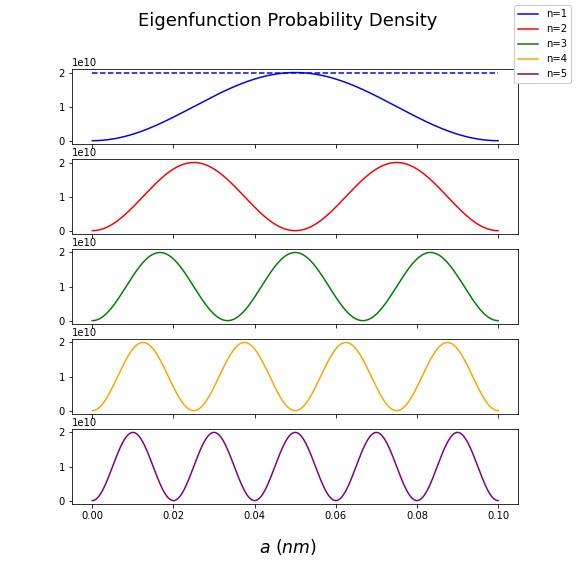
\includegraphics[width=0.6\textwidth]{lab1/probabilityDensity.png} %MISSING Y AXIS
    \caption{probability density for n=1 to n=5}
    \label{fig:probDens}
\end{figure}

The eigenstates of the system plotted above are stationary. This means that when the system is in one of these eigenstates, all quantum mechanical observables are conserved in time (probability $P=|\Psi(x,t)|^2dx$ is independent of $\phi(t)$, meaning $P=|\psi(x)|^2dx$).

On the other hand, superpositons of eigenfunctions are not stationary. To observe their non-stationary behaviours, namely, their time evolution we must calculate the superposition state for two states. The wavefunction for one state is given by:

$$\Psi_n (x,t) = \Psi_n (x)\Phi_n (t)$$
where $\Psi_n (x)= \sqrt{\frac{2}{a}} sin(\frac{\pi n}{a}x)$ and $\Phi_n (t)= e^{-i \omega t}$

The superposition state is therefore given by:
\begin{equation} \label{eq:superPos}
\Psi_s (x,t) = \Psi_n (x)e^{-i \omega_{1} t} + \Psi_m (x)e^{-i \omega_{2} t}
\end{equation}


This superposition wavefunction needs to be normalised, i. e.:

$$\int_{ -\infty}^{\infty} A^{*} \Psi_s (x)^{*} A\Psi_s (x)dx = 1$$
$$\left | A \right |^2 \int_{ -\infty}^{\infty} \Psi_s (x)^{*} \Psi_s (x)dx = 1$$

From Figure \ref{fig:particleInABox}:

$$\left | A \right |^2 \int_{0}^{a} \Psi_s (x)^{*} \Psi_s (x)dx = 1$$

Substituting Equation \ref{eq:superPos}

$$\left | A \right |^2 \int_{0}^{a} (\Psi_n (x)^{*}e^{i \omega_{1} t} + \Psi_m (x)^{*}e^{i \omega_{2} t}) (\Psi_n (x)e^{-i \omega_{1} t} + \Psi_m (x)e^{-i \omega_{2} t})dx = 1$$
$$\left | A \right |^2 \int_{0}^{a} (\left | \Psi_n (x) \right |^2 + \left | \Psi_m (x) \right |^2 + \Psi_n (x)^{*}\Psi_m (x)e^{-i(\omega_{2}- \omega_{1}) t} + \Psi_m (x)^{*}\Psi_n (x)e^{-i(\omega_{1}- \omega_{2}) t})dx = 1$$

$$ \left | A \right |^2 \int_{0}^{a}\left(\frac{2}{a} sin^{2}(\frac{\pi n_1}{a}x)+\frac{2}{a} sin^{2}(\frac{\pi n_2}{a}x)+\frac{2}{a} sin(\frac{\pi n_1}{a}x)sin(\frac{\pi n_2}{a}x)(e^{-i(\omega_{2}- \omega_{1})t}+e^{-i(\omega_{1}- \omega_{2})t})\right)dx = 1$$
$$...$$
$$\left | A \right |^2 \left( \frac{2}{a}\left(\frac{a}{2}\right) + \frac{2}{a}\left(\frac{a}{2}\right) + \frac{2}{a}(e^{-i(\omega_{2}- \omega_{1})t}+e^{-i(\omega_{1}- \omega_{2})t})\int_{0}^{a} sin(\frac{\pi n_1}{a}x)sin(\frac{\pi n_2}{a}x)dx \right)=1$$

$$\left | A \right |^2 \left( 1 + 1 + \frac{2}{a}(e^{-i(\omega_{2}- \omega_{1})t}+e^{-i(\omega_{1}- \omega_{2})t})(0) \right)=1$$
$$\left | A \right |^2 = \frac{1}{2}$$
$$\left | A \right | = \sqrt{\frac{2}{a}}$$
$$\therefore \Psi_s (x) = \sqrt{\frac{1}{2}} \left( \Psi_n (x)e^{-i \omega_{1} t} + \Psi_m (x)e^{-i \omega_{2} t}\right)$$

The real part of this superpositioned wavefunction was plotted as shown in Figure \ref{fig:superPosWave}.

\begin{figure}[h]
    \centering
    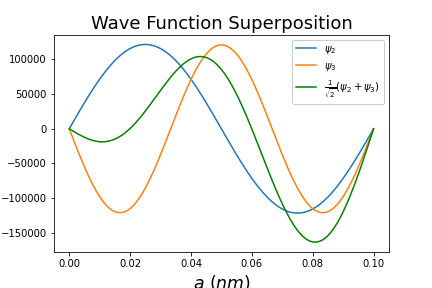
\includegraphics[width=0.75\textwidth]{lab1/superpositionWave.png}
    \caption{Plot two eigenstates, $\psi$ and $\psi$, and the superposition of both eigenstates}
    \label{fig:superPosWave}
\end{figure}

The probability distribution of the new wavefunction $\Psi_s(x,t)$ was then calculated and plotted at several different times to see how it evolves in time.

$$P_s(x, t) = |\Psi_s(x, t)|^{2} = A^{*} \Psi_s (x, t)^{*} A\Psi_s (x, t)$$
$$P_s(x) = \left | A \right |^2 \Psi_s (x)^{*} \Psi_s (x)$$
$$P_s(x) = 0.5 (\Psi_n (x)^{*}e^{i \omega_{1} t} + \Psi_m (x)^{*}e^{i \omega_{2} t}) (\Psi_n (x)e^{-i \omega_{1} t} + \Psi_m (x)e^{-i \omega_{2} t})$$
$$P_s(x) = 0.5 (\left | \Psi_n (x) \right |^2 + \left | \Psi_m (x) \right |^2 + \Psi_n (x)^{*}\Psi_m (x)e^{-i(\omega_{2}- \omega_{1}) t} + \Psi_m (x)^{*}\Psi_n (x)e^{i(\omega_{2}- \omega_{1}) t})$$
%n. b. $\Psi_n (x)=\Psi_n (x^{*})$ and $\Psi_m (x)=\Psi_m (x^{*})$
$$\therefore P_s(x) =  0.5 (\left | \Psi_n (x) \right |^2 + \left | \Psi_m (x) \right |^2 + \Psi_n (x)\Psi_m (x)e^{-i(\omega_{2}- \omega_{1}) t} + \Psi_m (x)\Psi_n (x)e^{i(\omega_{2}- \omega_{1}) t})$$
$$P_s(x) = 0.5 (\left | \Psi_n (x) \right |^2 + \left | \Psi_m (x) \right |^2 + \Psi_n (x)\Psi_m (x)(e^{-i(\omega_{2}- \omega_{1}) t} + e^{i(\omega_{2}- \omega_{1}) t}))$$
Since $cosx=\frac{e^{-i\omega x}+}{2}$ 
$$P_s(x) = 0.5 (\left | \Psi_n (x) \right |^2 + \left | \Psi_m (x) \right |^2 + \Psi_n (x)\Psi_m (x)(2cos\omega t))$$
$$P_s(x) = 0.5 \left | \Psi_n (x) \right |^2 + 0.5\left | \Psi_m (x) \right |^2 + \Psi_n (x)\Psi_m (x)cos\omega t$$

\begin{figure}[h]
    \centering
    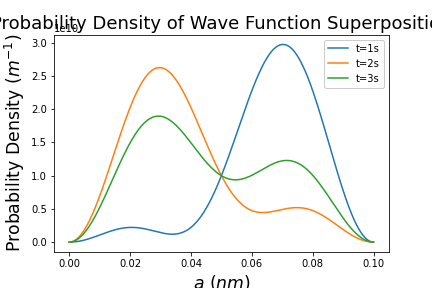
\includegraphics[width=0.75\textwidth]{lab1/superpositionPDF.png}
    \caption{Probability density function for the superimposed state for various times}
    \label{fig:superPosPDF}
\end{figure}

\section{Comparison of results with theory}

The results from this lab is entirely based on theory so there are no discrepancies of the results with theory.

To ensure this is true 

When calculating $E_n$ for $n=1,2,3,4,5$ it is clear to see that the ratio of $\frac{E_n}{E_1}$ is always equal to $n^{2}$ which agrees with Equation \ref{eq:energySpacing}. The energy levels must therefore become more sparse as $n$ increases, which can be seen in Figure \ref{fig:eigenEnergy}

All of the wave functions are 0 at each wall which means that the boundary conditions were always satisfied.

The peak wavefunctions $\approx \sqrt{2/L}$ and the peak probability is no higher than $2/L$.

The area under the probability density functions must always be equal to 1. To verify this the trap function was used.

Talk about plotting the real part and leaving out the imaginary part?


Also, the maximum of each wavefunction reaches the theoretical limit without surpassing it. The limit is:

$$ \text{Maximum}(|\Psi_n(x)|) = \sqrt{\frac{2}{L}} = \sqrt{\frac{2}{0.1e-9}} \approx  141421 $$

This is the necessary amplitude of the wave to achieve a normalised wavefunction.
The maximum of the wavefunction was found to be $141421$, \textbf{indicating that the plot is accurate. The same can be seen for Figure 1.3, where the theoretical limit is}:

$$ \text{Maximum}(|\Psi_n(x)|^{2}) = \frac{2}{L} = \frac{2}{0.1 \times 10^{-9}} = 2e^{10} $$

Again the peak value of the PDF was found to be $2e10$, \textbf{confirming the accuracy}.

\textbf{To confirm the PDF matches the theory and is being plotted correctly, it has to always satisfy the normalisation condition $\int_{0}^{a} |\Psi_s(x,t)|^{2} \,\delta x = 1$. By using the \textit{'trapz'} function to calculate an approximate area under the curve using the trapezium rule, it was found that the area ranged from 0.999998 to 1.000003 as $t$ progressed. The source of error comes from the intrinsic error of the trapezium rule and how the trapeziums cannot ever have infinitesimally small width}

Finally, by visual inspection we can see that the superposition is correct for all values of $t$. By choosing a location where one of $|\Psi_n(x)|$ or $|\Psi_m(x)| = 0$, we can see that the height of $|\Psi_s(x)|$ is $\frac{1}{\sqrt{2}}$ that of the non-zero wavefunction, thus confirming the superposition of the two is being calculated correctly. 

\section{Discussion}
\textbf{Question 1:}
After creating the energy-level diagram for up to $n=5$, create a code that finds the wavelengths of the photons emitted for all transitions beginning at state $n=3$ or less and ending at a lower energy state.

The wavelength was found using the following equation:

\[\lambda = \frac{hc}{\Delta E}\]
where $\lambda$ is the wavelength of the photon, $h$ is Planks constant, $c$ is the speed of light and $\Delta E$ is the difference in eigen energies.

\begin{lstlisting}[language=Python]
def wavelength(E):
    l = const.Planck*const.c/E
    return l

#Transition n=3 to n=2
print("n=3 to n=2 photon wavelength: ", 
      wavelength(Eigen_energies[2]-Eigen_energies[1]),"m")
#Transition n=3 to n=1
print("n=3 to n=1 photon wavelength: ", 
      wavelength(Eigen_energies[2]-Eigen_energies[0]),"m")
#Transition n=2 to n=1
print("n=2 to n=1 photon wavelength: ", 
      wavelength(Eigen_energies[1]-Eigen_energies[0]),"m")
\end{lstlisting}

\begin{lstlisting}[language=Python]
n=3 to n=2 photon wavelength:  6.594375173013399e-09 m
n=3 to n=1 photon wavelength:  4.1214844831333745e-09 m
n=2 to n=1 photon wavelength:  1.0990625288355668e-08 m
\end{lstlisting}

\section{Conclusions}